\chapter{Overhead-aware Workflow Model}
\label{chap:model}

In this chapter, we first introduce how we extend the existing DAG model to be overhead-aware. Second, we use our proposed model to describe the process of task clustering. 
%Second we present our overhead analysis on a series of widely used workflows, which is a base of our optimization methods that will be used in simulations. 
Third, we introduce the experiment environments used in this thesis including FutureGrid, a distributed platform and a workflow simulator as an example of the importance of an overhead model when simulating workflow execution. The simulation of a widely used workflow verifies the necessity of taking overheads into consideration.



\section{Overhead-aware DAG Model}

A DAG models the computational activities and data dependencies within a workflow and it fits with most workflow management systems such as Pegasus \cite{Deelman2004} and DAGMan \cite{Kalayci2010}. However, the preparation and execution of a scientific workflow in distributed environments often involve multiple components and the system overheads within and between these components cannot be ignored. 
An overhead is defined as the time of performing miscellaneous work other than executing computational activities. 
To address this challenge, in this thesis, we extend the existing Directed Acyclic Graph (DAG) model to be overhead-aware (o-DAG), in which an overhead is also a node in the DAG and the control dependencies are added as directed edges. We utilize o-DAG to provide a systematic analysis of the performance of workflow optimization methods and provide a series of novel optimization methods to further improve the overall workflow performance. 


%????
%Task clustering has been widely used in optimizing scientific workflows and can achieve significant improvement in the overall runtime performance \cite{Rynge2012, Singh2008, Li2011, Cao2008} of workflows. However,  there is a lack of a generic and systematic analysis and modeling of task clustering to improve the overall workflow performance including runtime, fault tolerance, data movement and resource utilization etc. 



\begin{figure}[h!]
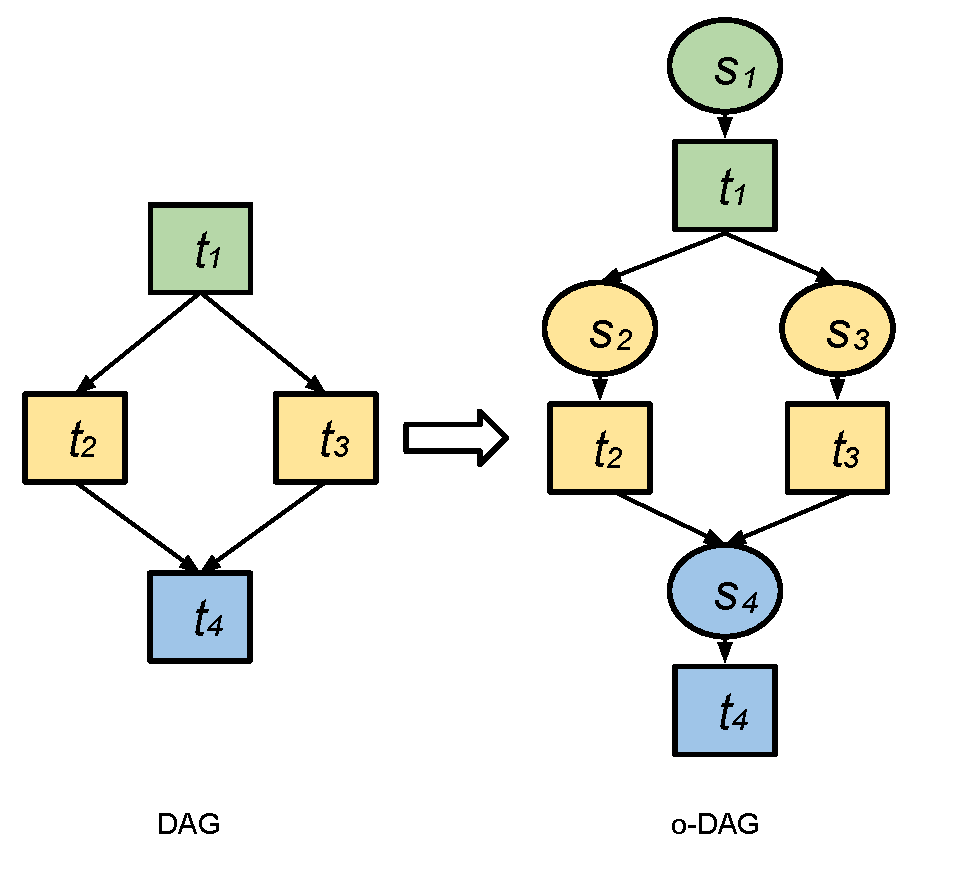
\includegraphics[width=0.6\linewidth]{figures/model/odag.pdf}
\centering
  \captionof{figure}{Extending DAG to o-DAG}
  \label{fig:model_odag}
\end{figure}

%In this work, we extend the DAG model to be overhead-aware (o-DAG). The reason is that system overheads play an important role in workflow execution and they constitute a major part of the overall runtime when tasks are poorly clustered. 
Fig~\ref{fig:model_odag} shows how we augment a DAG to be an o-DAG with the capability to represent scheduling overheads ($s$) such as workflow engine delay, queue delay, and postscript delay. The classification of these system overheads is based on the model of a typical workflow management system shown in Fig~\ref{fig:intro_system} and will be introduced in Section \ref{sec:overheads}. 


\subsection{Modeling Task Clustering}
\label{sec:task_clustering}

\begin{figure}[h!]
\centering
 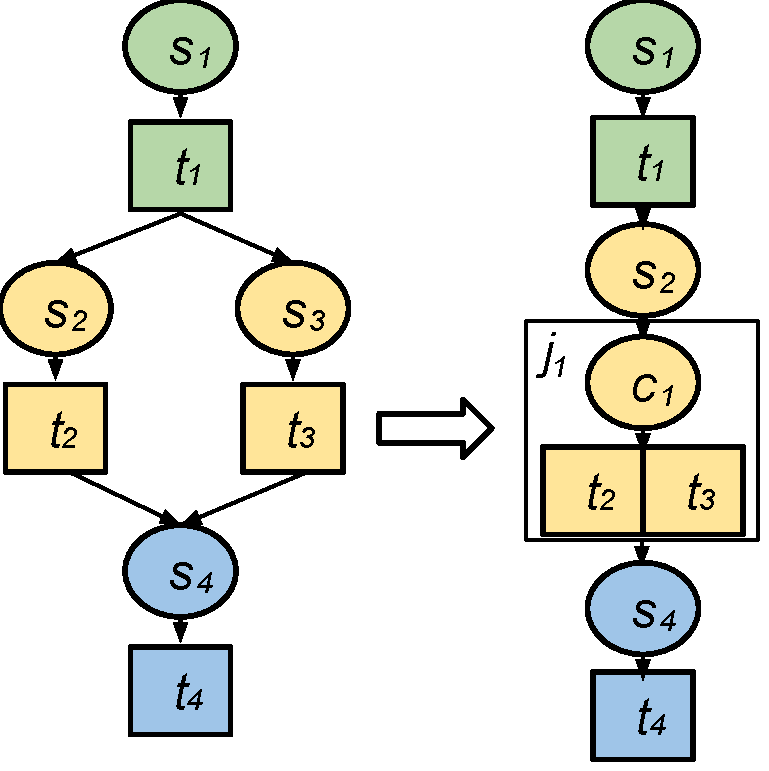
\includegraphics[width=0.5\linewidth]{figures/introduction/hc.pdf}
  \captionof{figure}{An example of task clustering (horizontal clustering)}
  \label{fig:intro_hc}
\end{figure}


\begin{figure}[!htb]
\centering
 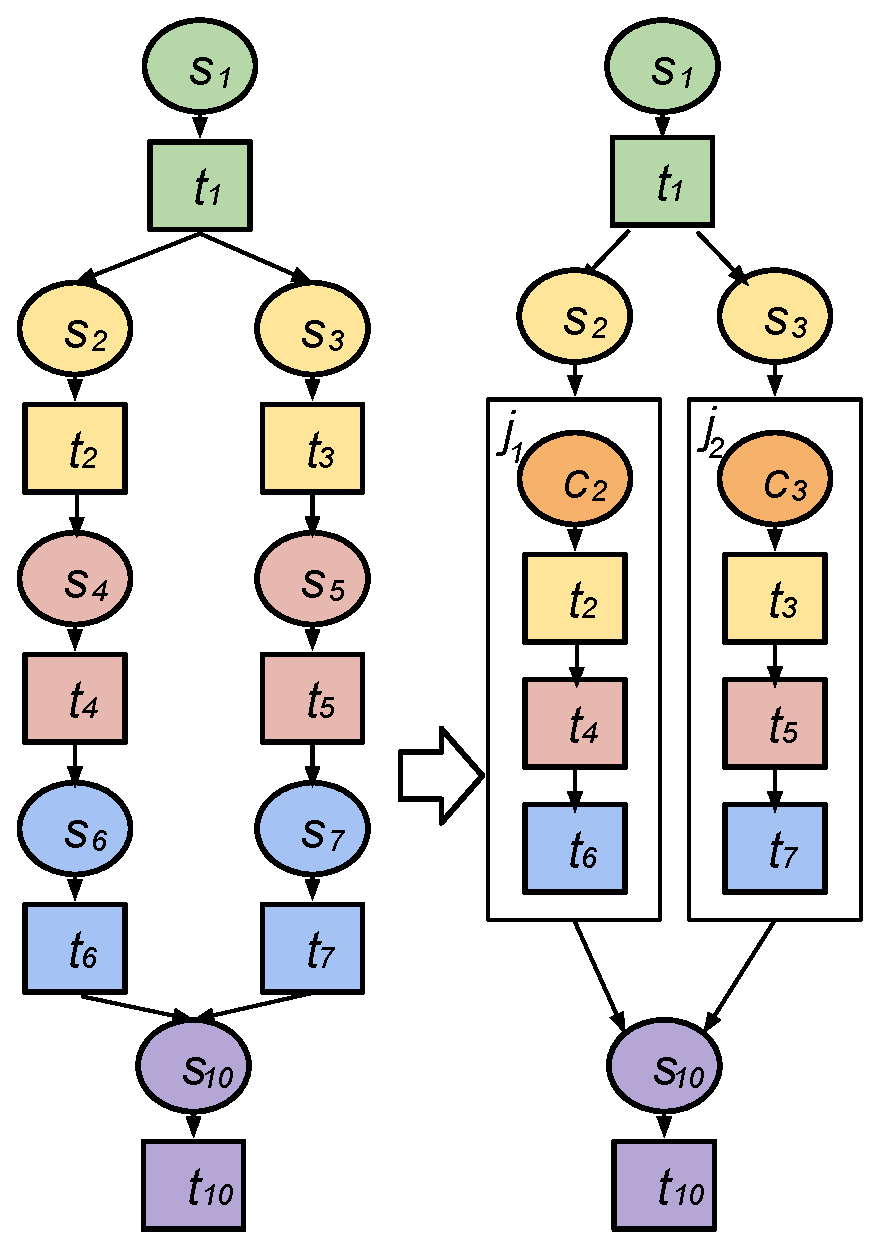
\includegraphics[width=0.5\linewidth]{figures/model/vc.pdf}
  \captionof{figure}{An example of vertical clustering.}
  \label{fig:model_vc}
\end{figure}

%Clustering delay ($c$) measures the difference between the sum of the actual task runtime and the job runtime seen by the job scheduler. The cause of clustering delay is usually the use of a job wrapper to execute a clustered job. 
%The job wrapper takes some time to extract the list of tasks and to launch them.

%With o-DAG model, we can explicitly express the process of task clustering. For example, in Fig~\ref{fig:intro_hc}, two tasks $t_2$ and $t_3$ without data dependency between them are merged into a clustered job $j_1$. Scheduling overheads ($s_3$) are reduced but clustering delay ($c_1$) is added. 

%A job ($j$) is a single execution unit and it contains one or multiple task(s). The process of merging tasks into a clustered job is called \textbf{task clustering}. 


With an o-DAG model, we can explicitly express the process of task clustering. In this thesis, we address task clustering horizontally and vertically. \textbf{Horizontal Clustering} (HC) merges multiple tasks that are at the same horizontal level of the workflow, in which the horizontal level of a task is defined as the longest distance from the entry task of the DAG to this task. \textbf{Vertical Clustering} (VC) merges tasks within a pipeline of the workflow. Tasks at the same pipeline share a single-parent-single-child relationship, which means a task $t_a$ is the unique parent of a task $t_b$, which is the unique child of $t_a$. 


Figure~\ref{fig:intro_hc} shows a simple example of how to perform HC, in which two tasks $t_2$ and $t_3$, without a data dependency between them, are merged into a clustered job $j_1$. A job is a single execution unit composed by one or multiple task(s). Job wrappers are commonly used to execute clustered jobs, but they add an overhead denoted by the clustering delay $c$. The clustering delay measures the difference between the sum of the actual task runtimes and the job runtime seen by the job scheduler. 
After horizontal clustering, $t_2$ and $t_3$ in $j_1$ can be executed in sequence or in parallel, if parallelism in one compute node is supported. In this work, we consider sequential executions only. Given a single resource, the overall runtime for the workflow in Figure~\ref{fig:intro_hc} (left) is $runtime_l= \sum_{i=1}^{4}(s_i+t_i)$, and the overall runtime for the clustered workflow in Figure~\ref{fig:intro_hc} (right) is $runtime_r=s_1+t_1+s_2+c_1+t_2+t_3+s_4+t_4$.  $runtime_l > runtime_r$ as long as $c_1 < s_3$, which is often the case in many distributed systems since the clustering delay within a single execution node is usually shorter than the scheduling overhead across different execution nodes. 


Figure~\ref{fig:model_vc} illustrates an example of vertical clustering, in which tasks $t_2$, $t_4$, and $t_6$ are merged into $j_1$, while tasks $t_3$, $t_5$, and $t_7$ are merged into $j_2$. Similarly, clustering delays $c_2$ and $c_3$ are added to $j_1$ and $j_2$ respectively, but system overheads $s_4$, $s_5$, $s_6$, and $s_7$ are removed. 



\section{Evaluation Methodologies}
\label{sec:experiments}

In this section, we introduce the experiment environments to evaluate our approaches in this thesis. 
%In Chapter~\ref{chap:partitioning}, we use FutureGrid to evaluation our workflow partitioning techniques. 
To evaluate our techniques in Chapter~\ref{chap:balance} and Chapter~\ref{chap:tolerance}, we have developed WorkflowSim, a trace based workflow simulator extended from CloudSim~\cite{Calheiros2011}. 
%We first introduce FutureGrid, a distributed cloud platform and then WorkflowSim, a traced based simulator developed by us. 
Below we introduce the details of WorkflowSim and we verify the effectiveness of WorkflowSim. 




\subsection{Overview of WorkflowSim}

We have developed WorkflowSim as an open source workflow simulator that extends CloudSim \cite{Calheiros2011} by providing a workflow level support of simulation. It models workflows with an o-DAG model with support of an elaborate model of node failures, a model of delays occurring in the various levels of the WMS stack \cite{Chen2011}, the implementations of several most popular dynamic and static workflow schedulers (e.g., HEFT\cite{Topcuoglu2002} and MinMin\cite{Blythe2005}) and task clustering algorithms (e.g., runtime-based algorithms \cite{Chen2013b}, data-oriented algorithms \cite{Chen2013b} and fault tolerant clustering algorithms \cite{Chen2012}). Parameters are imported from traces of workflow executions that were run on FutureGrid~\cite{Fox2013FutureGrid}. 

%However, an accurate simulation framework for scientific workflows is required to generate reasonable results, particularly considering that the overall system overhead \cite{Chen2011} plays a significant role in the workflow’s runtime. 
In distributed systems, workflows may experience different types of overheads.  Since the causes of overheads differ, the overheads have diverse distributions and behaviors. For example, the time to run a post-script that checks the return status of a computation is usually a constant. However, queue delays incurred while tasks are waiting in a batch scheduling systems can vary widely. 
By classifying these workflow overheads in different layers and system components, our simulator can offer a more accurate result than simulators that do not include overheads in their system models.

What’s more, many researchers \cite{Zhang2004, Tang1990, Schroeder2006, Sahoo2004, Oppenheimer2002, McConnel1979} have emphasized the importance of fault tolerant design and concluded that the failure rates in modern distributed systems should not be ignored. A simulation with support of random failures with different distributions is implemented in WorkflowSim to promote such studies. 

Finally, progress in workflow research also requires a general-purpose framework that can support widely accepted features of workflows and optimization techniques. Existing simulators such as CloudSim/GridSim \cite{Calheiros2011} fail to provide fine granularity simulations of workflows. For example, they lack the support of task clustering. The simulation of task clustering requires two layers of execution model, on both task and job levels. It also requires a workflow-clustering engine that launches algorithms and heuristics to cluster tasks. Other techniques such as workflow partitioning and task retry are also ignored in these simulators. These features have been implemented in WorkflowSim. 

To the best of our knowledge, none of the current distributed system simulators support these rich-features and techniques. Below, we introduce our early work on simulating scientific workflows satisfying these requirements. We evaluate the performance of WorkflowSim with an example of task clustering. 

\subsection{Components and Functionalities}

\begin{figure}[!htb]
	\centering
	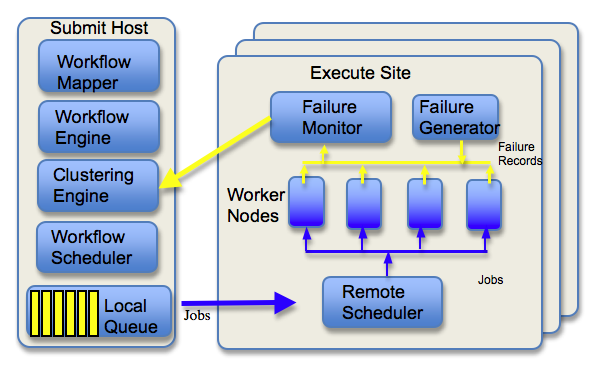
\includegraphics[width=0.6\linewidth]{figures/workflowsim/wfs_overview.png}
	\caption{Overview of WorkflowSim.}
	\label{fig:model_wfs}
\end{figure}

Deelman et. al. \cite{Deelman2009} have provided a survey of popular workflow systems for scientific applications and have classified their components into four categories: composition, mapping, execution, and provenance. Based on this survey, we identified the mandatory functionalities/components and designed the layers in our WorkflowSim. In our design as shown in Figure~\ref{fig:model_wfs}, we add multiple layers on top of the existing task scheduling layer of CloudSim, which include Workflow Mapper, Workflow Engine, Clustering Engine, Workflow Scheduler, Failure Generator and Failure Monitor etc. 

\begin{enumerate}

\item {Workflow Mapper} is used to import DAG files formatted in XML (called DAX in WorkflowSim) and other metadata information such as file size from Workflow Generator \cite{WorkflowGenerator}. Workflow Mapper creates a list of tasks and assigns these tasks to an execution site. A task is a program/activity that a user would like to execute. 

\item{Workflow Engine} manages tasks based on their dependencies between tasks to assure that a task may only be released when all of its parent tasks have completed successfully. Workflow Engine will only release free tasks to Clustering Engine. 

\item{Clustering Engine} merges tasks into jobs such that the scheduling overhead is reduced. A job is an atomic unit seen by the execution system, which contains multiple tasks to be executed in sequence or in parallel if applicable. Different to the clustering engine in Pegasus WMS, Clustering Engine in WorkflowSim also performs task reclustering in a faulty execution environment. The details will be introduced in Chapter \ref{chap:tolerance}. 

\item{Workflow Scheduler} is used to match jobs to a worker node based on the criteria selected by users. WorkflowSim relies on CloudSim to provide an accurate and reliable job-level execution model, such as time-shared model and space-shared model. However, WorkflowSim has introduced different layers of system overheads and failures, which improves the accuracy of simulation. 

\item{Failure Generator} is introduced to inject task/job failures at each execution site during the simulation. After the execution of each job, Failure Generator randomly generates task/job failures based on the distribution that a user has specified. 

\item{Failure Monitor} collects failure records (e.g., resource id, job id, task id) and returns these records to Clustering Engine to adjust the clustering strategies dynamically. 

\end{enumerate}




\subsection{Results and Validation}
We use task clustering as an example to illustrate the necessity of introducing system overheads into workflow simulation. The goal was to compare the simulated overall runtime of workflows in case the information of job runtime and system overheads are known and extracted from prior traces. 
In this example, we collected real traces generated by the Pegasus Workflow Management System while executing workflows on FutureGrid \cite{Fox2013FutureGrid}. We built an execution site with 20 worker nodes and we executed the Montage workflow five times in every single configuration of $clusters.num$, which is the maximum number of clustered jobs in a horizontal level. These five traces of workflow execution with the same $clusters.num$ is a training set or a validation set. 
%Partly illustrated by Figure 5, the results are stable enough to be used as a training set. 
We ran the Montage workflow with a size of 8-degree squares of sky. The workflow has 10,422 tasks and 57GB of overall data. We tried different $clusters.num$ from 20 to 100, leaving us 5 groups of data sets with each group having 5 workflow traces. 
First of all, we adopt a simple approach that selects a training set to train WorkflowSim and then use the same training set as validation set to compare the predicted overall runtime and the real overall runtime in the traces. We define accuracy in this section as the ratio between the predicted overall runtime and the real overall runtime:
\begin{equation} \label{eq:model_wfs_accuracy}
Accuracy=\frac{Predicted~Overall~Runtime}{Real~Overall~Runtime}
\end{equation}
 \begin{figure}[h!]
	\centering
    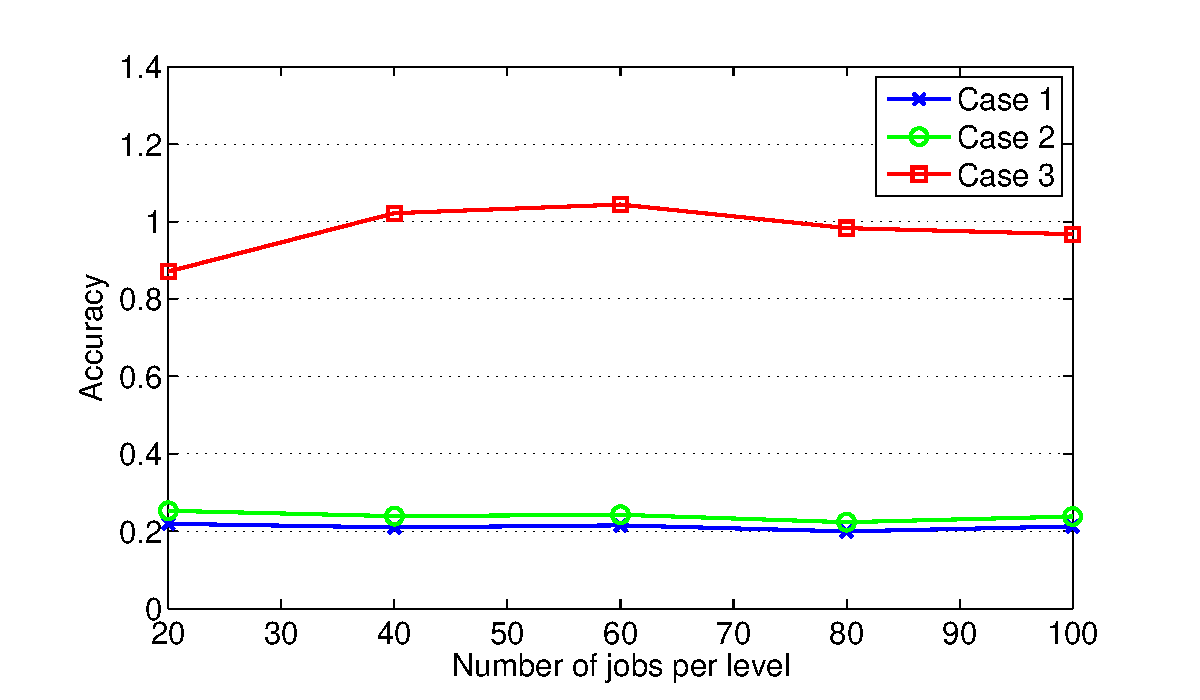
\includegraphics[width=0.7\textwidth]{figures/model/wfs_levels.eps}
    \caption{Performance of WorkflowSim with different support levels}
    \label{fig:model_wfs_levels}
\end{figure} 
 
%Performance of WorkflowSim with different support levels. 
To train WorkflowSim, from the traces of workflow execution (training sets), we extracted information about job runtime and overheads, such as average/distribution and, for example, whether it has a cyclic increase. We then added these parameters into the generation of system overheads and simulated them as close as possible to the real cases. 

To present an explicit comparison, we simulated the cases using WorkflowSim that has no consideration of workflow dependencies or overheads (Case 1), WorkflowSim with Workflow Engine that has considered the influence of dependencies but ignored system overheads (Case 2), and WorkflowSim, that has covered both aspects (Case 3). Intuitively, we expect that the order of the accuracy of them should be Case 3 $>$ Case 2 $>$ Case 1. 

Fig~\ref{fig:model_wfs_levels} shows that the performance of WorkflowSim with different support levels is consistent to our expectation. The accuracy of Case 3 is quite close to but not equal to 1.0 in most points. The reason is that to simulate workflows, WorkflowSim has to simplify models with a few parameters, such as the average value and the distribution type. It is not efficient to recur every overhead as is present in the real traces. It is also impossible to do so since the traces within the same training set may have much variance in each run. Fig~\ref{fig:model_wfs_levels} also shows that the accuracy of both Case 1 and Case 2 are much lower than that of Case 3. The reason is that it ignores both dependencies and multiple layers of overheads. By ignoring data dependencies, it releases tasks that are not supposed to run since their parents have not completed (a real workflow system should never do that) and thereby reducing the overall runtime. At the same time, it executes jobs/tasks irrespective of the actual overheads, which further reduces the simulated overall runtime. In Case 2, with the help of Workflow Engine, WorkflowSim is able to control the release of tasks and thereby the simulated overall runtime is closer to the real traces. However, since it has ignored most overheads, jobs are completed and returned earlier than that in real traces. The low accuracy of Case 1 and Case 2 confirms the necessity of introducing overhead design into our simulator. 


\section{Summary}

In this chapter, we have introduced an overhead-aware DAG model that we have proposed and the evaluation methodologies including a workflow simulator that we have developed. In next chapter, we will introduce the first proposed approach called Workflow Partitioning to address the optimization of workflows with resource constraints.

